\documentclass[10pt]{beamer}

\usepackage[utf8]{inputenc}
\usepackage[T5]{fontenc}
\usepackage[vietnamese]{babel}

\usetheme[progressbar=frametitle]{metropolis}
\usecolortheme{default}
\setbeamertemplate{footline}[frame number]

\usepackage{graphicx}
\graphicspath{{../baocao/figures/}{./}}
\usepackage{booktabs}
\usepackage{amsmath}
\usepackage{xcolor}
\usepackage{listings}
\usepackage{array}

\definecolor{accentRed}{HTML}{990000}
\setbeamercolor{title separator}{fg=accentRed}
\setbeamercolor{progress bar}{fg=accentRed,bg=accentRed!30}
\setbeamercolor{alerted text}{fg=accentRed}

\lstset{
  language=Python,
  basicstyle=\ttfamily\scriptsize,
  keywordstyle=\color{blue!70!black}\bfseries,
  commentstyle=\color{green!40!black},
  stringstyle=\color{orange!50!black},
  numbers=left,
  numberstyle=\tiny\color{gray},
  stepnumber=1,
  numbersep=6pt,
  frame=single,
  rulecolor=\color{black!20},
  breaklines=true,
  showstringspaces=false,
  tabsize=2
}

\title{Rút trích dữ liệu và tiền xử lý\\dữ liệu Pima Indians Diabetes}
\subtitle{Báo cáo học phần thay thế khóa luận}
\author{Nhóm 01}
\institute{Khoa Toán Ứng dụng - Trường Đại học Sài Gòn}
\date{\today}
\titlegraphic{\hfill
\includegraphics[height=0.8cm]{logohcmut.png}}

\begin{document}

\begin{frame}
  \titlepage
\end{frame}

\begin{frame}{Mục tiêu buổi trình bày}
  \begin{itemize}
    \item Trình bày đầy đủ quy trình nghiên cứu từ dữ liệu đến kết quả mô hình.
    \item Giải thích rõ các quyết định kỹ thuật (missing ẩn, imputation, scaling, baseline).
    \item Tổng hợp insight thực nghiệm để trả lời trực tiếp các câu hỏi nghiên cứu.
    \item Đưa ra kết luận, hạn chế và khuyến nghị triển khai trong thực tế.
  \end{itemize}
\end{frame}

\begin{frame}{Outline}
  \tableofcontents
\end{frame}

\section{Chương 1 - Tổng quan vấn đề}

\begin{frame}{Lý do chọn đề tài}
  \begin{itemize}
    \item Đái tháo đường là bệnh mạn tính có xu hướng gia tăng và nhiều biến chứng nặng.
    \item Nhu cầu sàng lọc sớm đòi hỏi cách tiếp cận định lượng, tái lập và nhất quán.
    \item Dữ liệu y sinh thực tế có nhiễu, missing ẩn và quan hệ đa biến phức tạp.
    \item Học máy phù hợp để mô hình hóa xác suất nguy cơ, hỗ trợ quyết định ban đầu.
  \end{itemize}
  \vspace{0.3em}
  \textbf{Bộ dữ liệu lựa chọn:} Pima Indians Diabetes (benchmark kinh điển).
\end{frame}

\begin{frame}{Mục tiêu và câu hỏi nghiên cứu}
  \textbf{Mục tiêu chính}
  \begin{itemize}
    \item Xây dựng pipeline phân tích dữ liệu y sinh có khả năng tái lập.
    \item So sánh các chiến lược \textit{imputer + scaler + model} trong cùng điều kiện.
    \item Tối ưu quyết định vận hành thông qua phân tích threshold trade-off.
  \end{itemize}
  \vspace{0.4em}
  \textbf{3 câu hỏi cốt lõi}
  \begin{enumerate}
    \item \textit{zero-as-missing} có cải thiện kết quả không?
    \item Tổ hợp preprocessing + model nào phù hợp nhất?
    \item Precision/Recall biến thiên thế nào khi thay đổi threshold?
  \end{enumerate}
\end{frame}

\begin{frame}{Đối tượng, phạm vi và luồng tổng quát}
  \begin{itemize}
    \item Dữ liệu: 768 mẫu, 8 biến đầu vào, nhãn nhị phân \texttt{outcome}.
    \item Phạm vi: EDA, tiền xử lý, baseline (Logistic Regression, Random Forest).
    \item Không bao gồm: deep learning, external dataset, tuning quy mô lớn.
  \end{itemize}
  \begin{block}{Luồng kỹ thuật}
    Khảo sát dữ liệu $\rightarrow$ xử lý missing ẩn $\rightarrow$ EDA $\rightarrow$ pipeline tiền xử lý
    $\rightarrow$ huấn luyện baseline $\rightarrow$ đánh giá đa chỉ số và phân tích ngưỡng.
  \end{block}
\end{frame}

\section{Chương 2 - Cơ sở lý thuyết và nghiên cứu liên quan}

\begin{frame}{Khung lý thuyết bài toán phân lớp y sinh}
  \begin{itemize}
    \item Bài toán phân lớp nhị phân: dự đoán \texttt{outcome} \(\in \{0,1\}\).
    \item Dữ liệu tabular y sinh có:
      \begin{itemize}
        \item phân phối lệch,
        \item outlier và missing ẩn,
        \item tương tác biến không thuần tuyến tính.
      \end{itemize}
    \item Hiệu năng mô hình phụ thuộc mạnh vào chất lượng tiền xử lý.
  \end{itemize}
\end{frame}

\begin{frame}{Xử lý dữ liệu: zero-as-missing, imputation, scaling}
  \textbf{Zero-as-missing}
  \begin{itemize}
    \item Chuyển các giá trị \texttt{0} phi sinh lý ở \texttt{glucose, blood\_pressure, skin\_thickness, insulin, bmi} thành missing.
  \end{itemize}
  \textbf{Imputation}
  \begin{itemize}
    \item Median, KNN, Iterative (MICE).
  \end{itemize}
  \textbf{Scaling}
  \begin{itemize}
    \item StandardScaler và MinMaxScaler để đồng nhất thang đo.
  \end{itemize}
\end{frame}

\begin{frame}{Mô hình baseline và chỉ số đánh giá}
  \begin{columns}[T,totalwidth=\textwidth]
    \column{0.52\textwidth}
    \textbf{Mô hình}
    \begin{itemize}
      \item Logistic Regression: baseline tuyến tính, dễ diễn giải.
      \item Random Forest: mô hình phi tuyến, bắt tương tác biến tốt.
    \end{itemize}
    \column{0.48\textwidth}
    \textbf{Chỉ số}
    \begin{itemize}
      \item Accuracy
      \item Precision
      \item Recall
      \item F1-score
      \item ROC-AUC
    \end{itemize}
  \end{columns}
  \begin{alertblock}{Lưu ý}
    Với bài toán sàng lọc, Recall và F1 thường quan trọng hơn Accuracy đơn lẻ.
  \end{alertblock}
\end{frame}

\section{Chương 3 - Dữ liệu và phương pháp đề xuất}

\begin{frame}{Nguồn dữ liệu và thuộc tính}
  \begin{itemize}
    \item \texttt{Lab\_03/data/pima-indians-diabetes.csv}
    \item \texttt{Lab\_03/data/pima-indians-diabetes.names}
  \end{itemize}
  \vspace{0.3em}
  \begin{table}
    \centering
    \scriptsize
    \begin{tabular}{p{2.6cm}p{4.8cm}}
      \toprule
      \textbf{Biến tiêu biểu} & \textbf{Ý nghĩa} \\
      \midrule
      \texttt{glucose} & Nồng độ glucose huyết tương \\
      \texttt{insulin} & Nồng độ insulin huyết thanh \\
      \texttt{bmi} & Chỉ số khối cơ thể \\
      \texttt{age} & Tuổi bệnh nhân \\
      \texttt{outcome} & Nhãn phân lớp (0/1) \\
      \bottomrule
    \end{tabular}
  \end{table}
\end{frame}

\begin{frame}{Kiểm tra chất lượng dữ liệu}
  \begin{columns}[T,totalwidth=\textwidth]
    \column{0.58\textwidth}
    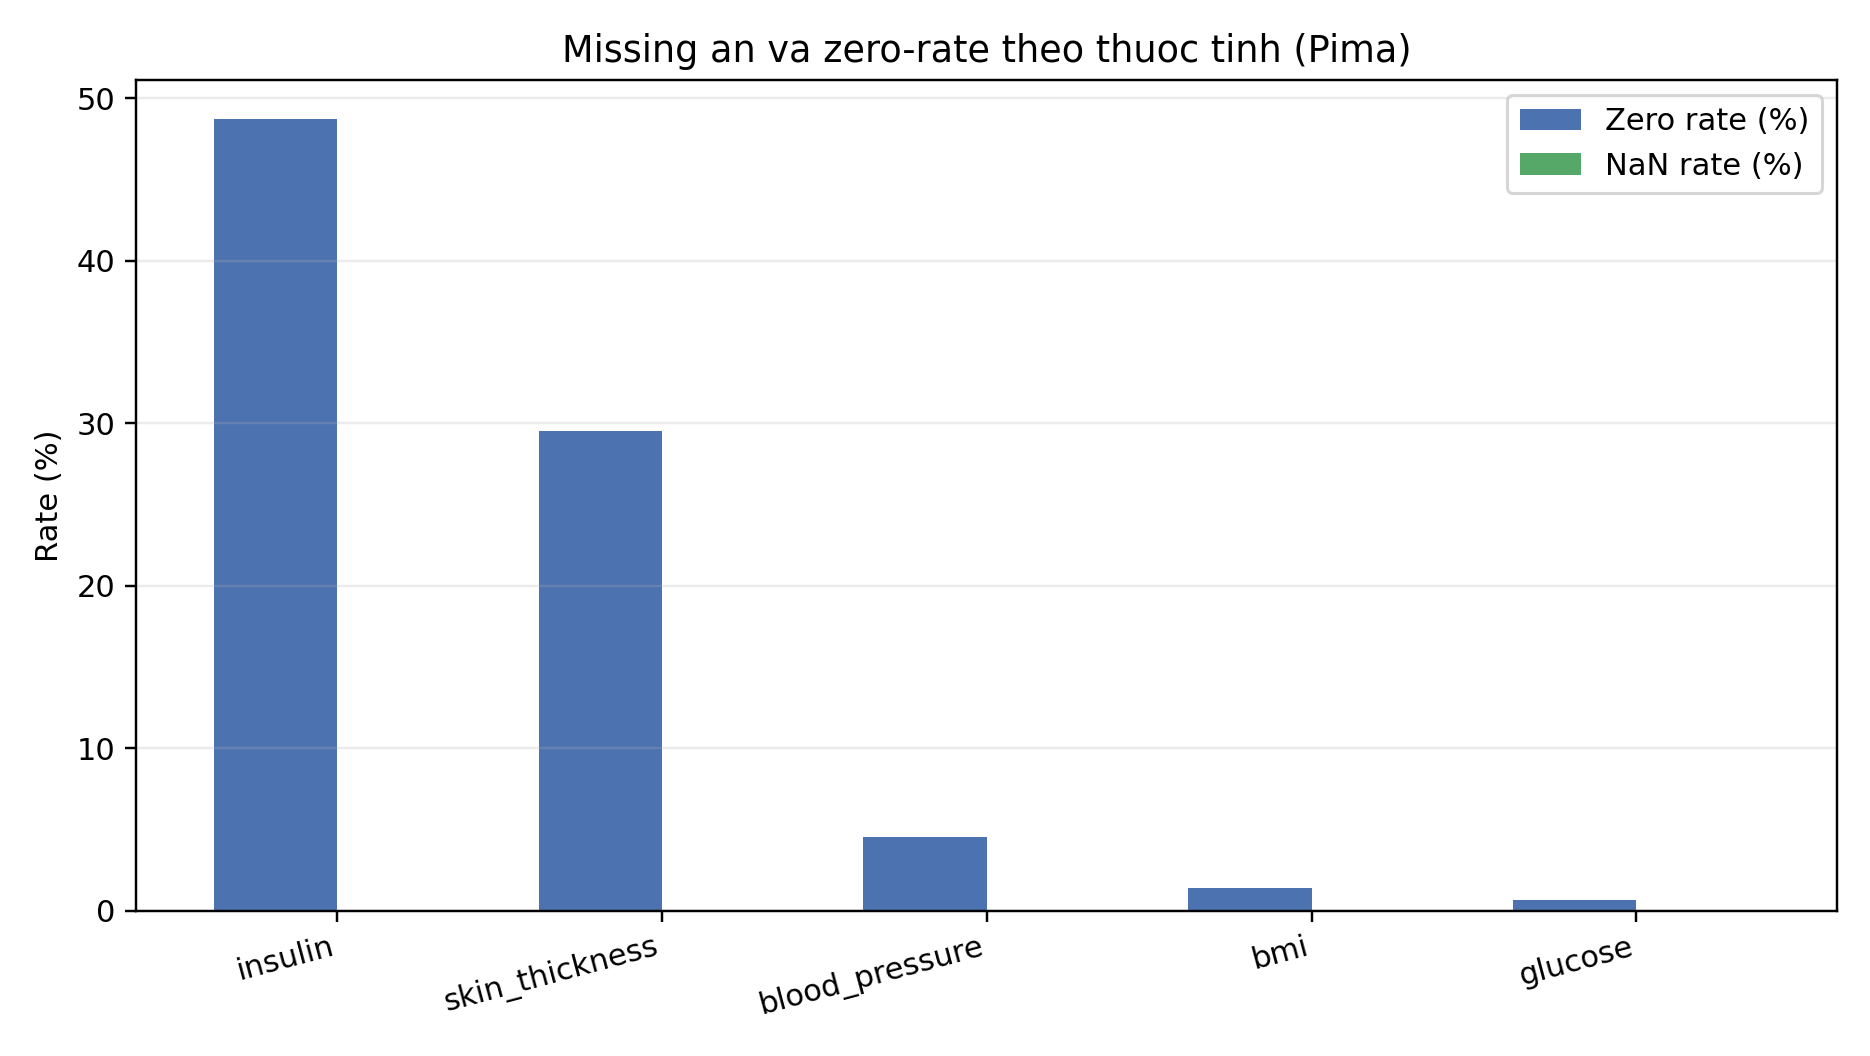
\includegraphics[width=\linewidth]{fig_missing_zero_report.png}
    \column{0.42\textwidth}
    \textbf{Nhận xét chính}
    \begin{itemize}
      \item Không có dòng trùng lặp.
      \item Không có NaN tường minh trong file gốc.
      \item Missing ẩn tập trung ở \texttt{insulin}, \texttt{skin\_thickness}.
      \item Cần chuyển \texttt{0} bất thường thành missing trước huấn luyện.
    \end{itemize}
  \end{columns}
\end{frame}

\begin{frame}[fragile]{Code block: chia dữ liệu có stratify}
\begin{lstlisting}
X = df[feature_columns].copy()
y = df["outcome"].astype(int)
X[zero_as_missing_columns] = X[zero_as_missing_columns].replace(0, np.nan)

X_train_val, X_test, y_train_val, y_test = train_test_split(
    X, y, test_size=0.2, random_state=42, stratify=y
)
X_train, X_val, y_train, y_val = train_test_split(
    X_train_val, y_train_val, test_size=0.25,
    random_state=42, stratify=y_train_val
)
\end{lstlisting}
  \textbf{Insight:} Chia 2 bước giúp đạt đúng tỉ lệ 60/20/20 và giữ ổn định tỷ lệ lớp dương trên mọi tập.
\end{frame}

\begin{frame}[fragile]{Code block: pipeline baseline}
\begin{lstlisting}
Pipeline(steps=[
  ("imputer", SimpleImputer(strategy="median")),
  ("scaler", StandardScaler()),
  ("clf", LogisticRegression(max_iter=5000, random_state=42))
])
\end{lstlisting}
  \begin{itemize}
    \item Tất cả phép biến đổi được fit trên train.
    \item Giảm data leakage và tăng tính tái lập.
    \item Dễ mở rộng sang nhiều cấu hình khác nhau.
  \end{itemize}
\end{frame}

\begin{frame}{EDA chuyên sâu theo nhóm biến}
  \begin{columns}[T,totalwidth=\textwidth]
    \column{0.33\textwidth}
    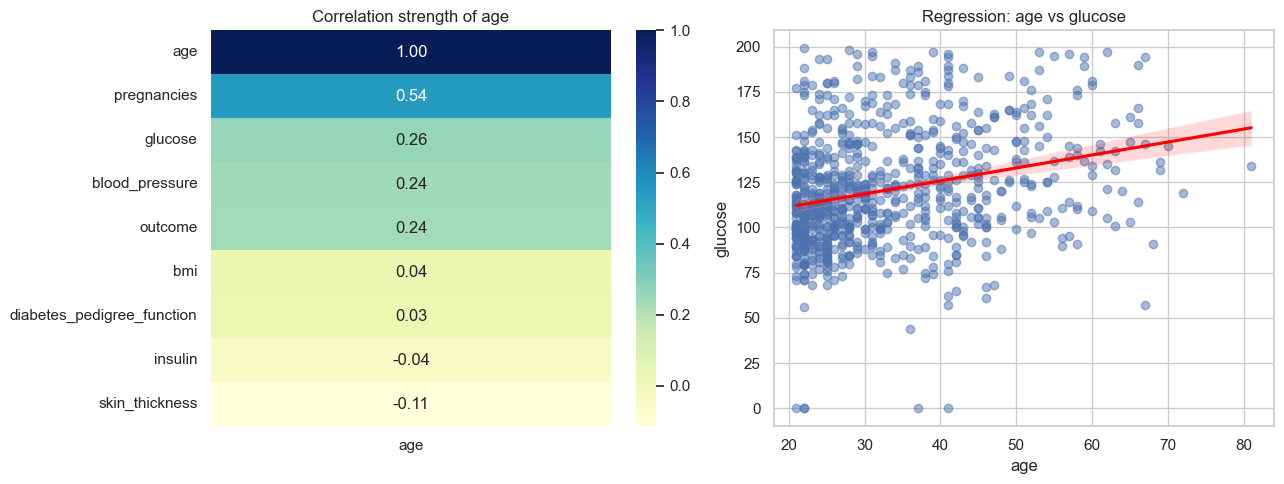
\includegraphics[width=\linewidth]{age_glucose_correlation.png}
    \column{0.33\textwidth}
    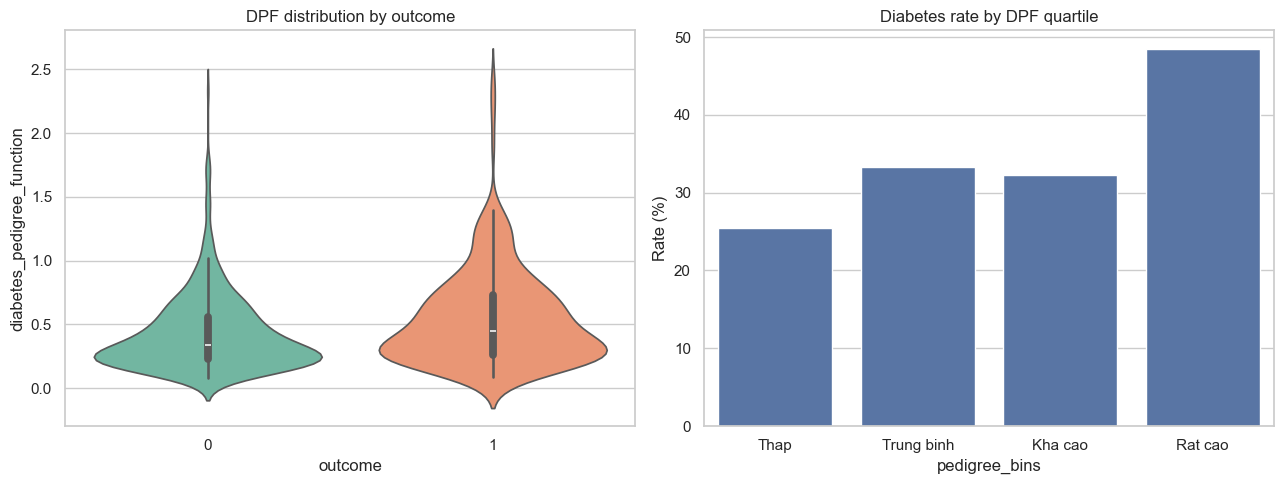
\includegraphics[width=\linewidth]{dpf_and_focus_scatter.png}
    \column{0.33\textwidth}
    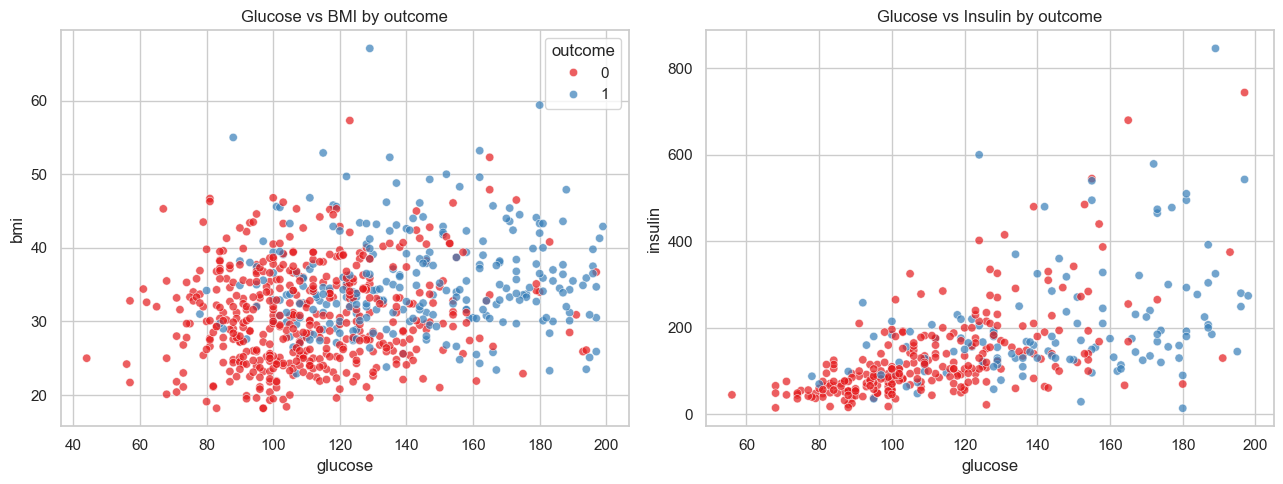
\includegraphics[width=\linewidth]{glucose_bmi_insulin_scatter.png}
  \end{columns}
  \vspace{0.4em}
  \begin{itemize}
    \item \texttt{glucose} thể hiện khả năng phân tách lớp rõ nhất.
    \item DPF, BMI, insulin bổ sung tín hiệu rủi ro khi kết hợp đa biến.
    \item Quan hệ không thuần tuyến tính $\Rightarrow$ cần so sánh mô hình phi tuyến.
  \end{itemize}
\end{frame}

\begin{frame}{Pipeline tiền xử lý đề xuất}
  \begin{columns}[T,totalwidth=\textwidth]
    \column{0.55\textwidth}
    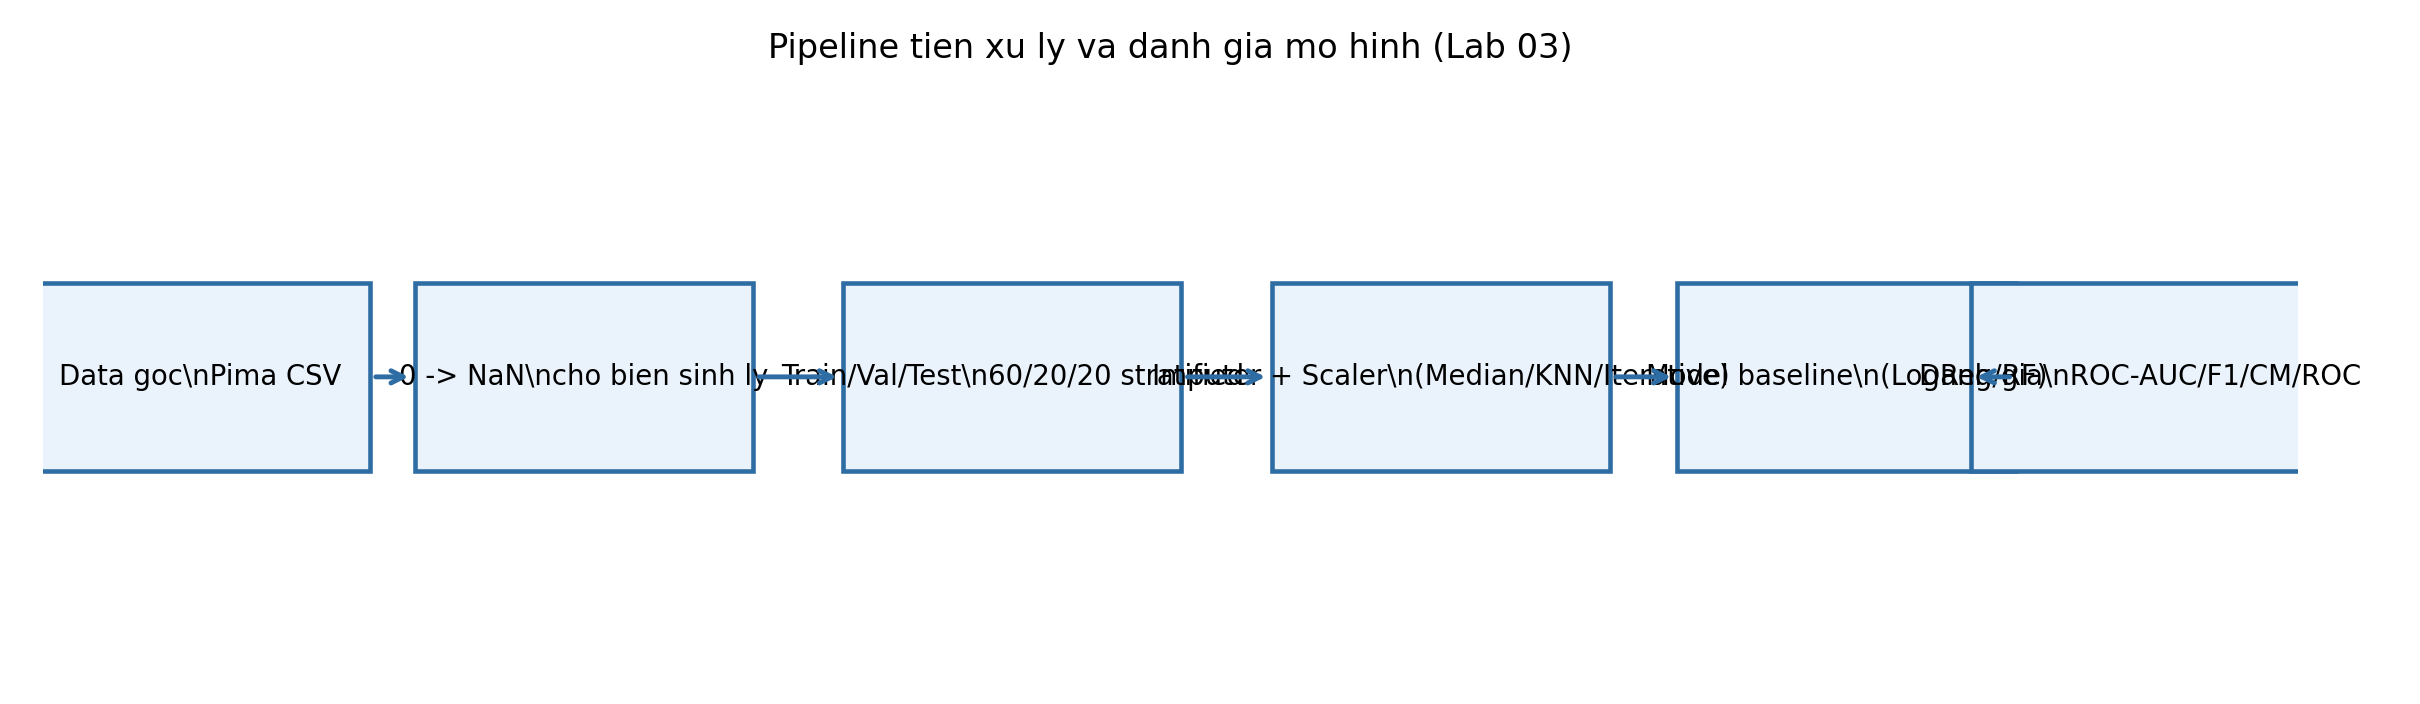
\includegraphics[width=\linewidth]{fig_preprocess_pipeline.png}
    \column{0.45\textwidth}
    \begin{enumerate}
      \item Chuẩn hóa dữ liệu đầu vào.
      \item Xử lý missing ẩn.
      \item Imputation.
      \item Scaling.
      \item Huấn luyện + đánh giá.
    \end{enumerate}
    \vspace{0.2em}
    \textbf{Thông điệp:} Quy trình thống nhất giúp so sánh công bằng và giảm lỗi thao tác thủ công.
  \end{columns}
\end{frame}

\section{Chương 4 - Thực nghiệm và kết quả đạt được}

\begin{frame}{Thiết lập thực nghiệm}
  \textbf{Chiến lược chia dữ liệu}
  \begin{itemize}
    \item Train: 460 mẫu
    \item Validation: 154 mẫu
    \item Test: 154 mẫu
  \end{itemize}
  \textbf{Không gian so sánh}
  \begin{itemize}
    \item Imputation: Median, KNN, Iterative
    \item Scaling: Standard, MinMax
    \item Model: Logistic Regression, Random Forest
  \end{itemize}
  \textbf{Tổng cộng:} 12 cấu hình trên cùng seed và cùng split.
\end{frame}

\begin{frame}{Phân bố lớp và tương quan chính}
  \begin{columns}[T,totalwidth=\textwidth]
    \column{0.48\textwidth}
    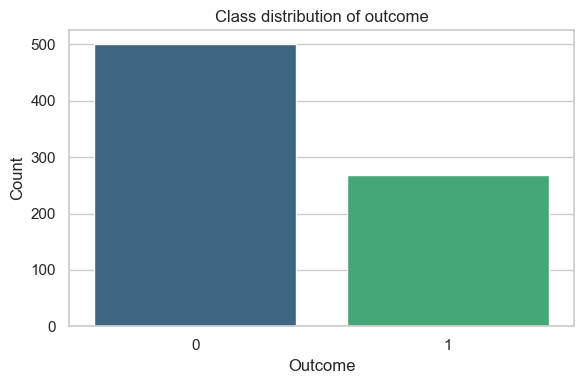
\includegraphics[width=\linewidth]{class_distribution.png}
    \column{0.48\textwidth}
    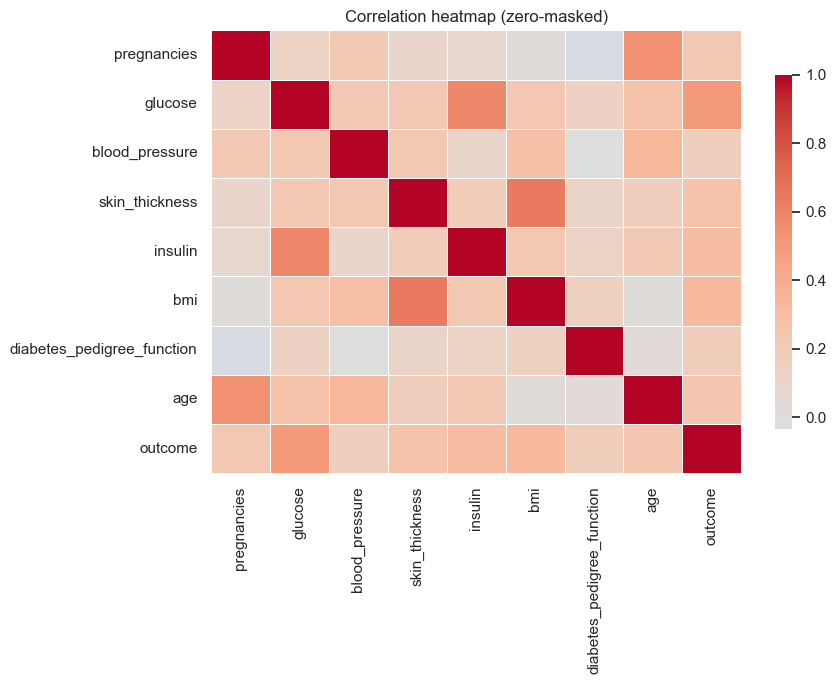
\includegraphics[width=\linewidth]{corr_heatmap.png}
  \end{columns}
  \vspace{0.4em}
  \begin{itemize}
    \item Lớp âm chiếm ưu thế nhẹ $\Rightarrow$ cần theo dõi Recall/F1.
    \item \texttt{glucose} có tương quan mạnh nhất với \texttt{outcome}.
    \item Không có biến đơn lẻ đủ quyết định nhãn $\Rightarrow$ cần mô hình đa biến.
  \end{itemize}
\end{frame}

\begin{frame}[fragile]{Code block: đánh giá một cấu hình}
\begin{lstlisting}
def evaluate_strategy(imputer_name, scaler_name, model_name):
    pipe = Pipeline([...])
    pipe.fit(X_train, y_train)
    y_val_pred = pipe.predict(X_val)
    y_val_prob = pipe.predict_proba(X_val)[:, 1]
    y_test_pred = pipe.predict(X_test)
    y_test_prob = pipe.predict_proba(X_test)[:, 1]
    return {
      "val_f1": f1_score(y_val, y_val_pred),
      "val_roc_auc": roc_auc_score(y_val, y_val_prob),
      "test_f1": f1_score(y_test, y_test_pred),
      "test_roc_auc": roc_auc_score(y_test, y_test_prob),
    }
\end{lstlisting}
  \textbf{Insight:} Mọi tổ hợp dùng cùng pipeline đánh giá, đảm bảo tính công bằng trong bảng xếp hạng.
\end{frame}

\begin{frame}{Kết quả 12 cấu hình (tóm tắt)}
  \scriptsize
  \begin{table}
    \centering
    \begin{tabular}{lllcc}
      \toprule
      \textbf{Imputer} & \textbf{Scaler} & \textbf{Model} & \textbf{Test AUC} & \textbf{F1}\\
      \midrule
      KNN & MinMax & Random Forest & 0.8170 & 0.6078\\
      KNN & Standard & Random Forest & 0.8168 & 0.6078\\
      Median & Standard & Logistic Reg. & 0.8167 & 0.5455\\
      Iterative & MinMax & Random Forest & 0.8156 & 0.5882\\
      \bottomrule
    \end{tabular}
  \end{table}
  \vspace{0.3em}
  \begin{itemize}
    \item Nhóm Random Forest ổn định hơn về F1.
    \item KNN Imputer thường xuất hiện ở top theo ROC-AUC.
  \end{itemize}
\end{frame}

\begin{frame}{So sánh chiến lược và cấu hình đề xuất}
  \begin{columns}[T,totalwidth=\textwidth]
    \column{0.56\textwidth}
    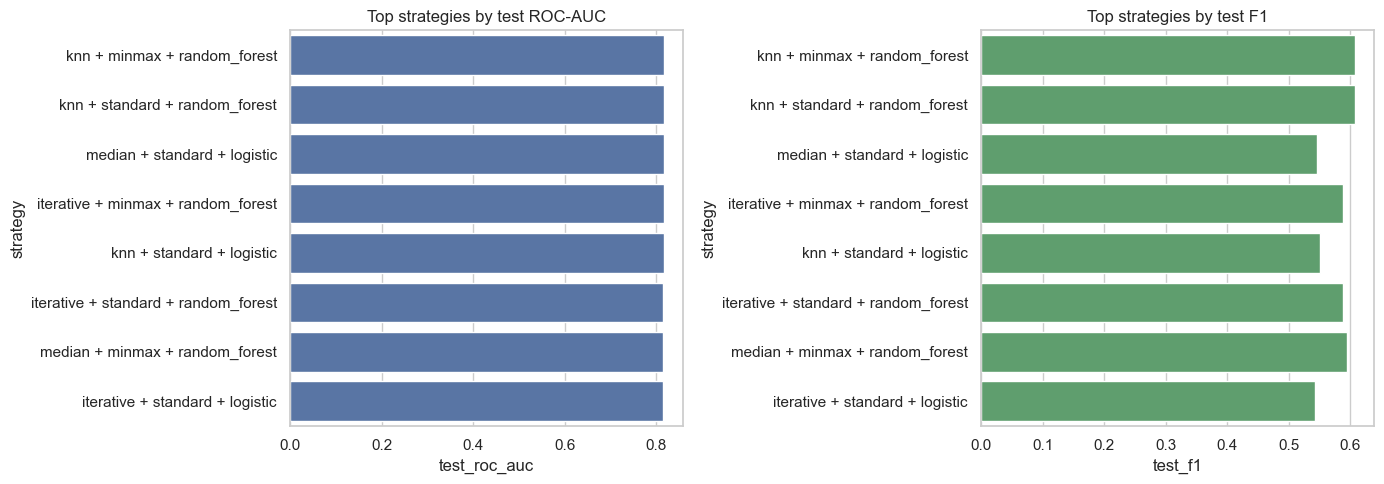
\includegraphics[width=\linewidth]{strategy_comparison.png}
    \column{0.44\textwidth}
    \textbf{Cấu hình đề xuất}
    \begin{itemize}
      \item KNN + MinMax + Random Forest
      \item Val AUC: 0.8700
      \item Test AUC: 0.8170
      \item Test F1: 0.6078
      \item Test Recall: 0.5741
    \end{itemize}
    \textbf{Nhận xét}
    \begin{itemize}
      \item AUC top khá sát nhau.
      \item Cần chọn theo mục tiêu nghiệp vụ, không chỉ theo 1 chỉ số.
    \end{itemize}
  \end{columns}
\end{frame}

\begin{frame}{Phân tích sai số: Confusion matrix + ROC}
  \begin{columns}[T,totalwidth=\textwidth]
    \column{0.5\textwidth}
    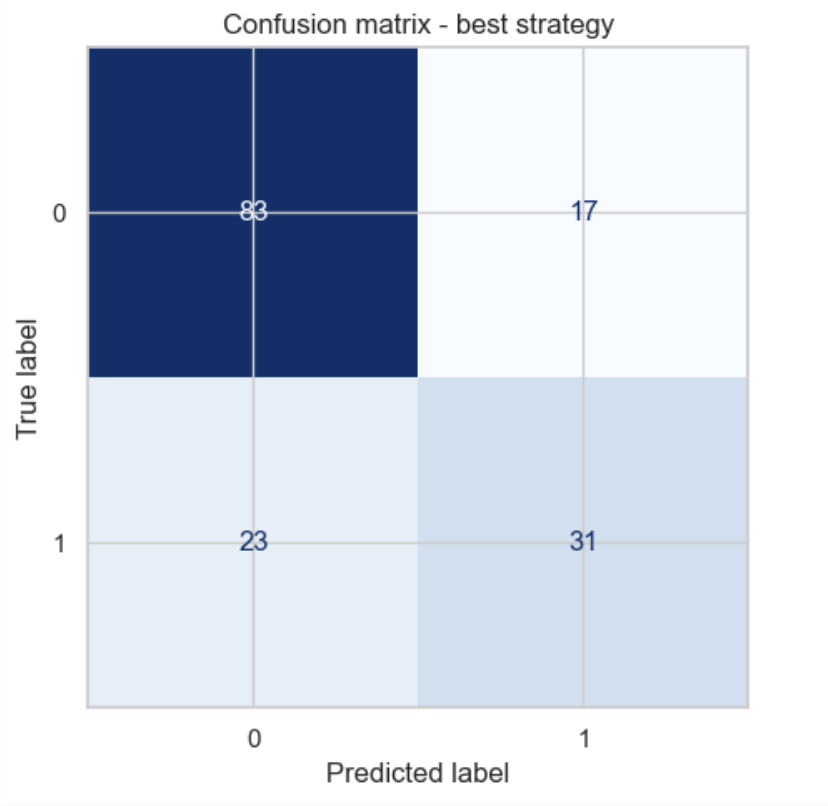
\includegraphics[width=\linewidth]{confusion_best.png}
    \column{0.5\textwidth}
    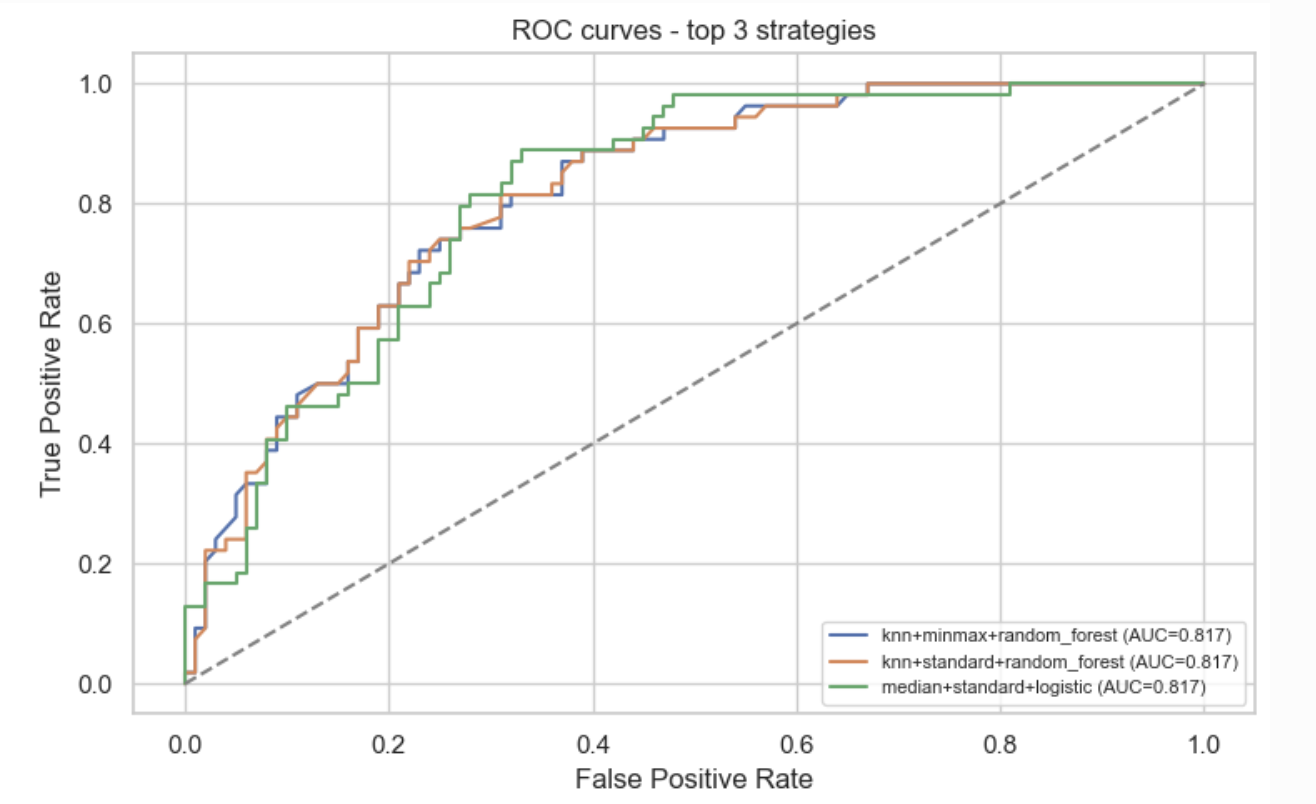
\includegraphics[width=\linewidth]{roc_top3.png}
  \end{columns}
  \vspace{0.3em}
  \begin{itemize}
    \item Tại ngưỡng 0.5: TN=86, FP=17, FN=23, TP=31.
    \item Vẫn bỏ sót ca dương đáng kể $\Rightarrow$ cần tối ưu threshold cho sàng lọc.
  \end{itemize}
\end{frame}

\begin{frame}[fragile]{Code block: quét threshold}
\begin{lstlisting}
thresholds = np.arange(0.30, 0.75, 0.05)
rows = []
for thr in thresholds:
    pred_thr = (best_artifacts["y_test_prob"] >= thr).astype(int)
    rows.append({
      "threshold": thr,
      "precision": precision_score(y_test, pred_thr),
      "recall": recall_score(y_test, pred_thr),
      "f1": f1_score(y_test, pred_thr),
    })
threshold_df = pd.DataFrame(rows)
\end{lstlisting}
\end{frame}

\begin{frame}{Trade-off theo threshold}
  \scriptsize
  \begin{table}
    \centering
    \begin{tabular}{cccc}
      \toprule
      Threshold & Precision & Recall & F1 \\
      \midrule
      0.30 & 0.5789 & 0.8148 & 0.6769 \\
      0.40 & 0.6167 & 0.6852 & 0.6491 \\
      0.50 & 0.6458 & 0.5741 & 0.6078 \\
      0.60 & 0.6944 & 0.4630 & 0.5556 \\
      0.70 & 0.7500 & 0.3333 & 0.4615 \\
      \bottomrule
    \end{tabular}
  \end{table}
  \begin{alertblock}{Kết luận vận hành}
    Ngưỡng 0.30 phù hợp hơn cho pha sàng lọc ban đầu vì Recall cao (0.8148), chấp nhận đánh đổi Precision.
  \end{alertblock}
\end{frame}

\section{Chương 5 - Kết luận và khuyến nghị}

\begin{frame}{Kết luận chính}
  \begin{enumerate}
    \item \textit{zero-as-missing} có tác động thực chất đến chất lượng mô hình.
    \item KNN + MinMax + Random Forest cho test ROC-AUC cao nhất.
    \item Random Forest ổn định hơn Logistic Regression về F1 trong dữ liệu phi tuyến.
    \item Điều chỉnh threshold giúp cải thiện mạnh mục tiêu sàng lọc.
  \end{enumerate}
\end{frame}

\begin{frame}{Trả lời trực tiếp Q1/Q2/Q3}
  \textbf{Q1 -- Zero-as-missing có hữu ích không?}\\
  Có, giúp giảm nhiễu từ giá trị phi sinh lý và ổn định AUC quanh 0.81 trên test.
  \vspace{0.4em}

  \textbf{Q2 -- Tổ hợp tốt nhất?}\\
  KNN Imputer + MinMaxScaler + Random Forest.
  \vspace{0.4em}

  \textbf{Q3 -- Trade-off theo threshold?}\\
  Giảm threshold từ 0.5 xuống 0.3 làm Recall tăng rõ (0.5741 $\rightarrow$ 0.8148),
  F1 cũng tăng (0.6078 $\rightarrow$ 0.6769).
\end{frame}

\begin{frame}{Đóng góp, hạn chế và khuyến nghị}
  \textbf{Đóng góp}
  \begin{itemize}
    \item Chuẩn hóa pipeline tái lập từ EDA đến đánh giá baseline.
    \item Cung cấp benchmark 12 cấu hình trong cùng điều kiện thực nghiệm.
  \end{itemize}
  \textbf{Hạn chế}
  \begin{itemize}
    \item Dữ liệu nhỏ (768 mẫu), chưa có external validation.
    \item Chưa tuning hệ thống và chưa calibration xác suất.
  \end{itemize}
  \textbf{Khuyến nghị}
  \begin{itemize}
    \item Ngắn hạn: Stratified K-Fold + tuning + calibration.
    \item Trung hạn: thử boosting và kỹ thuật cân bằng lớp.
    \item Dài hạn: mở rộng dữ liệu, đóng gói pipeline triển khai.
  \end{itemize}
\end{frame}

\appendix
\section{Phụ lục}

\begin{frame}{Bảng đầy đủ 12 cấu hình (appendix)}
  \tiny
  \begin{tabular}{lllcc}
    \toprule
    Imputer & Scaler & Model & Test AUC & F1\\
    \midrule
    KNN & MinMax & Random Forest & 0.8170 & 0.6078\\
    KNN & Standard & Random Forest & 0.8168 & 0.6078\\
    Median & Standard & Logistic Regression & 0.8167 & 0.5455\\
    Iterative & MinMax & Random Forest & 0.8156 & 0.5882\\
    KNN & Standard & Logistic Regression & 0.8154 & 0.5510\\
    Iterative & Standard & Random Forest & 0.8153 & 0.5882\\
    Median & MinMax & Random Forest & 0.8149 & 0.5941\\
    Iterative & Standard & Logistic Regression & 0.8148 & 0.5417\\
    Median & Standard & Random Forest & 0.8136 & 0.5941\\
    KNN & MinMax & Logistic Regression & 0.8117 & 0.5474\\
    Median & MinMax & Logistic Regression & 0.8098 & 0.5532\\
    Iterative & MinMax & Logistic Regression & 0.8093 & 0.5567\\
    \bottomrule
  \end{tabular}
\end{frame}

\begin{frame}[standout]
  Cảm ơn thầy/cô và các bạn đã theo dõi.
\end{frame}

\end{document}
